\documentclass[../sdrg,../../main.tex]{subfiles}
\begin{document}
\section{Dasgupta-Ma RG Method for the Heisenberg Model}
Most generally, the Heisenberg model with random couplings and anisotropy is 

\begin{equation}
    H=\sum_{i}^{N}\vec{J}_{i}\vec{S}_{i}\vec{S}_{i+1}
\end{equation}

The coupling constants $J_{i}$ show quenched randomness, meaning they are randomly distributed in space, but fixed in time, following a certain distribution function $P(J),\ 0<J<\max{J}=\Omega$. Because of this, the chain does not have translational invariance which causes the system to not have a spin-wave spectrum. It is therefore easier (if not the only possible way) to find approximate solutions for the problem of arbitrary $P(J)$.\\

If we want to decimate a general random XYZ chain, we have to pick the bond with the largest of the possible $J$. Without loss of generality, we name that bond the $n=2$ bond, so the local Hamiltonian takes the form
\begin{equation}
    \mathcal{H}_{23}=\vec{J}_{2}\vec{S}_{2}\vec{S}_{3}
\end{equation}

Because the bond $2-3$ is the strongest, we are able to handle the bonds $1-4$ pertubatively, which is shown in Appendix B. This means that the $1-4$ Hamiltonian is of the form
\begin{equation}
    \mathcal{H}_{14}=E_{14}'+\vec{J}'_{14}\vec{S}'_{1}\vec{S}'_{4}
\end{equation}
where 
\begin{equation}
\label{eq:recursionrel}
J_{1-4}^{x}=\frac{J_{1}^{x} J_{3}^{x}}{J_{2}^{y}+J_{2}^{z}}
\end{equation}
the approximated pertubation of the bond in the x direction\footnote{Likewise for $J_{1-4}^{y.z}$.}.
By ignoring the stable term\footnote{The stable term would be useful to calculate things such as the ground energy, but in general can be emitted.}, and by taking the $\vec{J}_{1,3}<<\vec{J}_{2}$, we get that $\tilde{S}_{1,4}=S_{1,4}$ up to $\mathcal{O}(\flatfrac{J_{1,3}}{J{2}})$\cite{fisher} and therefore the effective Hamiltonian in (3.3) will yield the correct ground energy, low-energy spectrum, and low-temperature correlation functions of $S_1$ and $S_4$. We shall use the recursion relation \eqref{eq:recursionrel} as the basis for the renormalisation group transformations for the rest of the chapter.\\

% \begin{figure}[h!]
%     \centering
%     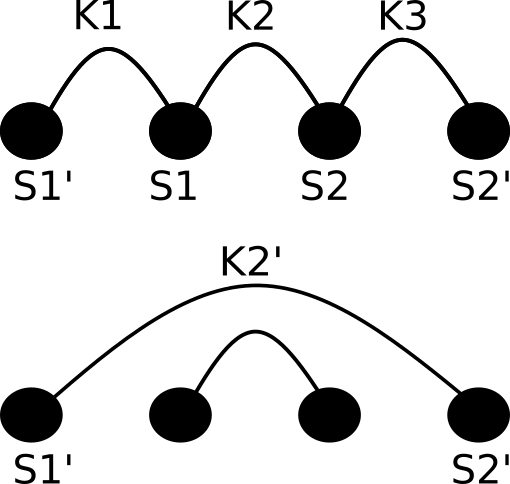
\includegraphics[scale=0.3]{Chapter4/Figures/RG.png}
%     \caption{The process of a single iteration of the RG method.}
%     \label{fig:elimtrans}
% \end{figure}

The flow equation takes the form of
\begin{equation}
    \pdv{P}{J}=R[P]
\end{equation}
where $R[P]$ is a complex functional.
\end{document}